\section{A first Kalman filter and its properties}
\subsection{a}

Generate the data points using the method from the small pre-tasks.

\begin{figure}[H]
 \centering
 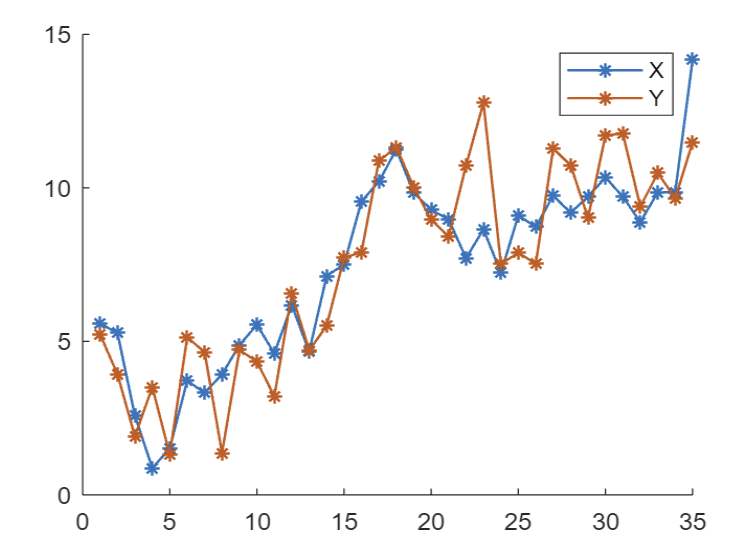
\includegraphics[width=0.7\textwidth]{images/figurefor1a.png}
 \caption{capital}
 \label{1a}
\end{figure}

From figure \ref{1a}, we can see that measurement Y is basically following the trend of model state X. 

The 'matrix' A and H in this scenario are scalar 1, which means the curve of Y and the curve of X should coincide without noises, while there exist motion and measurement noises and the covariance of \emph{R} is high compared to \emph{Q}, some Y and X are very widely separated.

\subsection{b}


\begin{figure}[H]
    \centering
    \begin{subfigure}[b]{0.45\textwidth}
        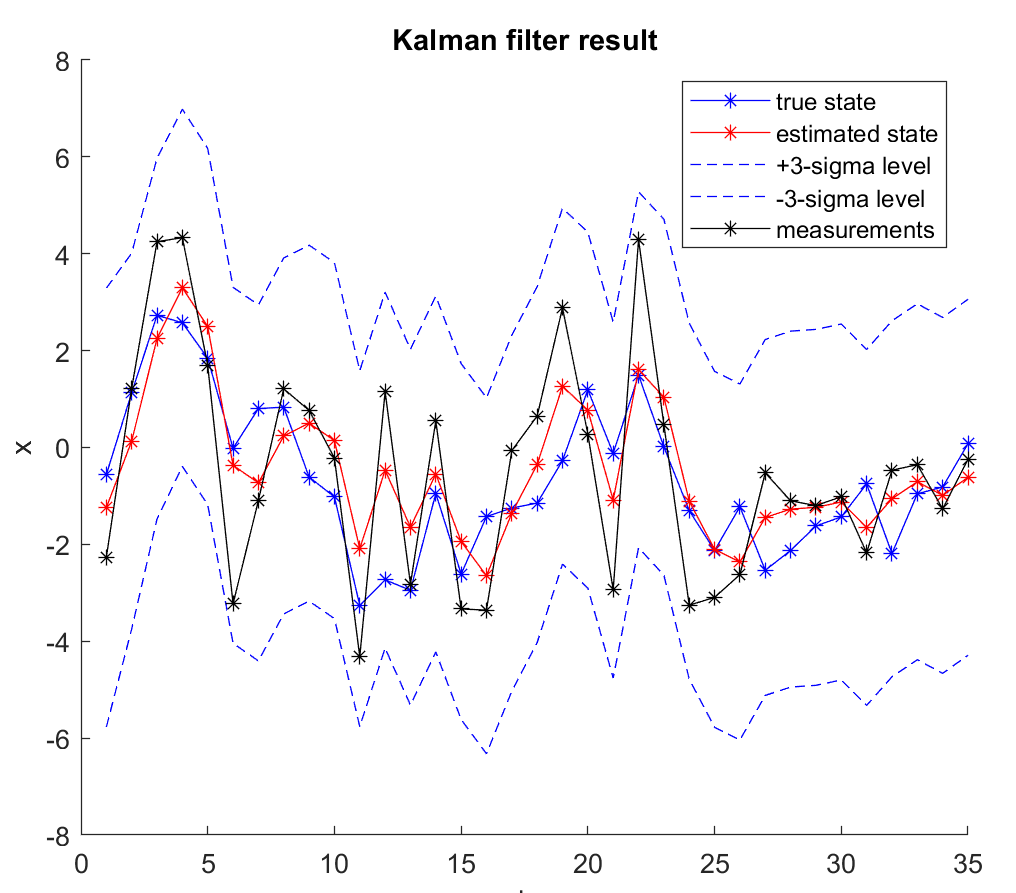
\includegraphics[width=\textwidth]{images/kalmanfilterresult.png}
        \caption{Kalman filter result}
        \label{1b1}
    \end{subfigure}
    \hfill
    \begin{subfigure}[b]{0.45\textwidth}
        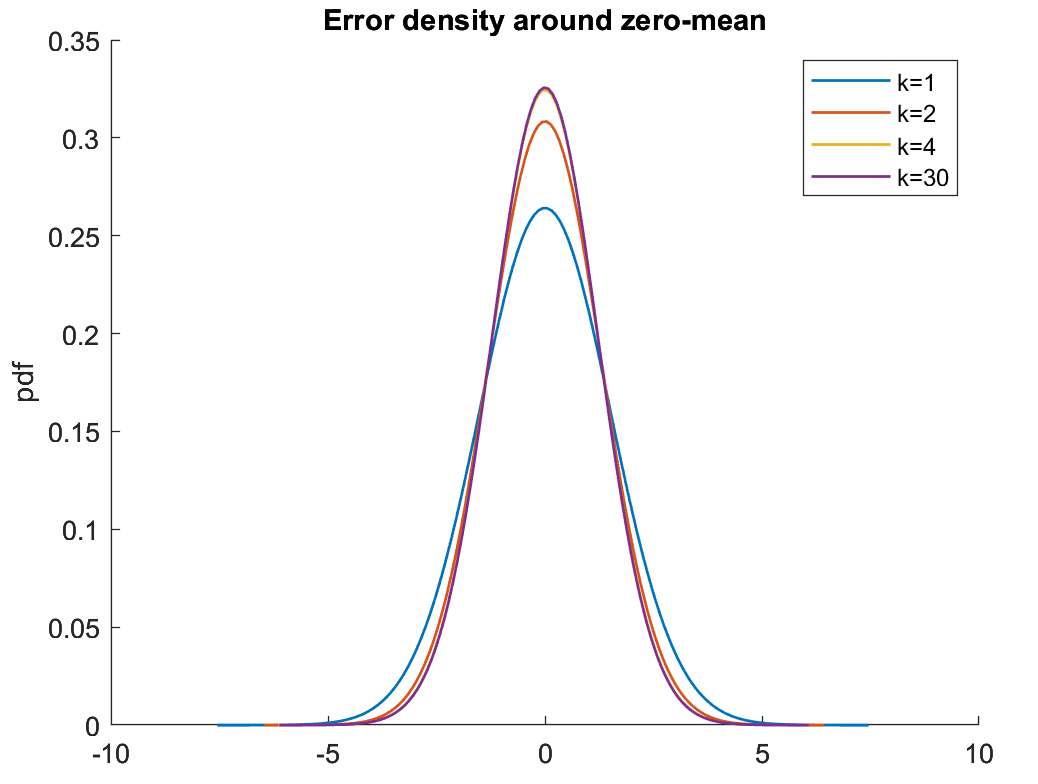
\includegraphics[width=\textwidth]{images/errordensity.png}
        \caption{Error density around zero-mean}
        \label{1b2}
    \end{subfigure}
    \caption{Figures for 1b}
    \label{1b}
    \end{figure}
  
The first figure \ref{1b1} shows the result of the Kalman filter, where the blue line represents the true state sequence, the red line represents the estimated state sequence, the black asterisks represent the measurements, and the blue dashed lines represent the $+/-3 \sigma$ level of the estimated state sequence. As we can see, the estimated state sequence follows the true state sequence quite well and varies in a narrow zone. Since the measurement values nearly hit the $ 3 \sigma $ borders and the borders change following the trend of the true state, it means the uncertainty represented by the error covariance is reasonable.

The second figure \ref{1b2} shows the error density around zero-mean for time instances k = [1; 2; 4; 30]. The error density is represented by the Gaussian density with mean zero and standard deviation equal to the square root of the corresponding element of the error covariance matrix. As we can see, the error density becomes narrower and taller as the time instance k increases, which indicates that the uncertainty in the estimate decreases as we observe more measurements.

\subsection{c}
In this part, we give the Kalman filter a wrong prior and see what happens.

One thing that needs to care about here is that we only need to change the \emph{x\_0} for \texttt{kalmanFilter} because the true state is something really exists in the real world that does not change according to some wrong prior. The prior should only influence the filter.

\begin{figure}[H]
 \centering
 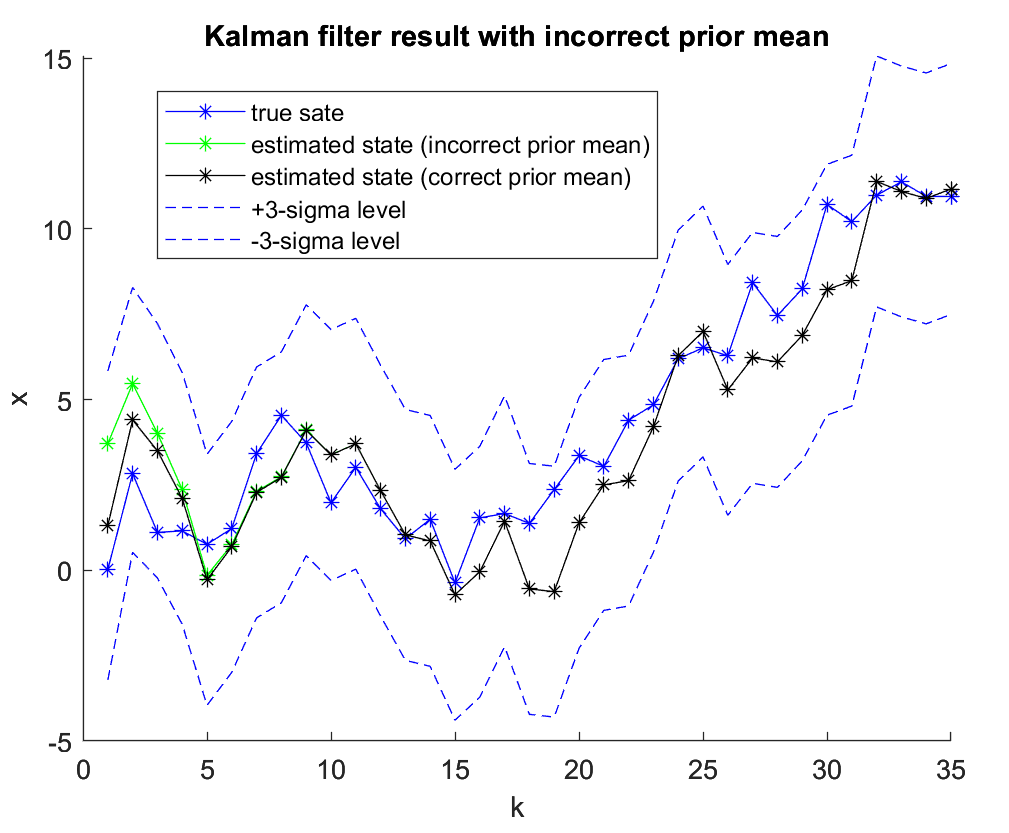
\includegraphics[width=0.7\textwidth]{images/incorrectpriorcompare.png}
 \caption{Kalman filter result with incorrect prior mean}
 \label{1c}
\end{figure}


In the plot, we can see that the estimates generated by the Kalman filter with the incorrect prior mean (green line) are initially far from the true states (blue line) and the true estimate state(black line). However, as more measurements are observed, the estimates converge toward the true states. After 10 new measurements, the incorrect estimate totally merges into the correct measurements. This means that while the estimates generated by the Kalman filter with the incorrect prior mean will deviate from the true states initially, they will become more accurate over time. If the time is long enough, there shouldn't be any difference between the incorrect estimate and the correct estimate.

\subsection{d}

\begin{figure}[H]
 \centering
 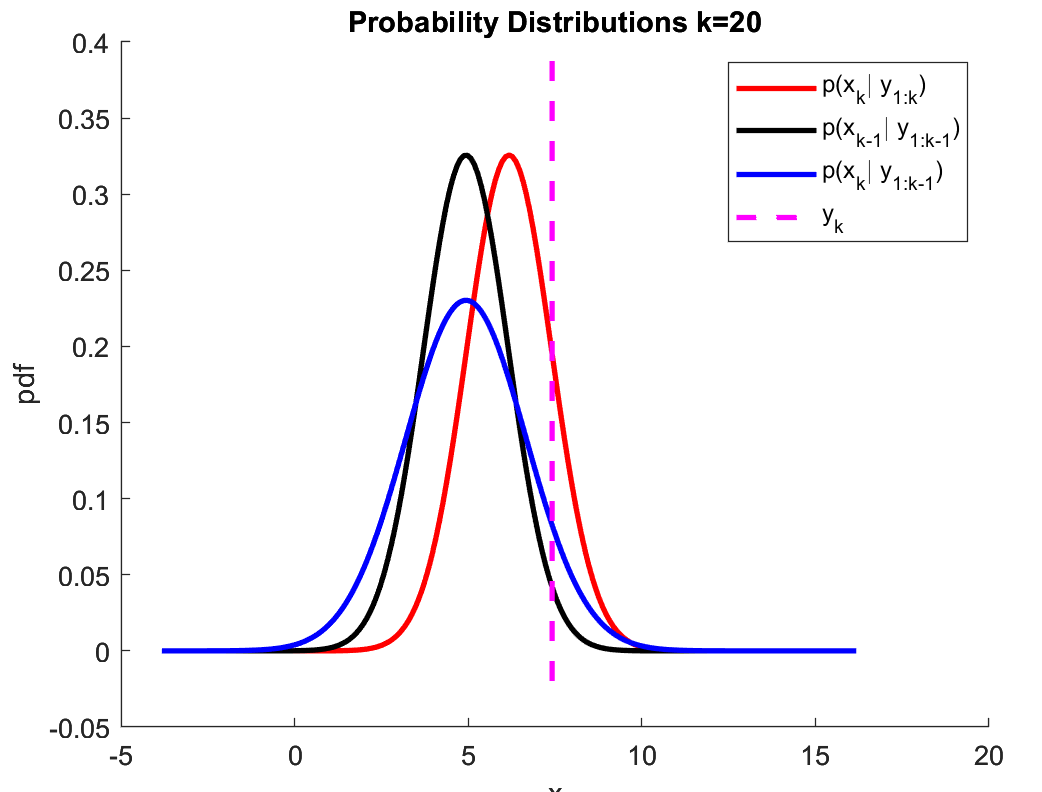
\includegraphics[width=0.7\textwidth]{images/steps.png}
 \caption{Four curves}
 \label{1d}
\end{figure}

In figure \ref{1d}, we can see a clear process of updating the probability distribution of the state.

Prior information is depicted by $p(x_{k-1}\big|y_{1:k-1})$, which is the black curve on the left.

The blue curve is $p(x_k\big|y_{1:k-1})$, the estimated probability, the prediction. From the figure, we can see it has more uncertainty than the prior and has the same mean with the prior.

The measurement, $ y_k $, the pink dotted line on the right, offers more information to us and gets to the current state posterior $p(x_k\big|y_{1:k})$. It 'drags' the prior curve to the right.

The red curve $p(x_{k}\big|y_{1:k})$ is posterior. We can see the mean of posterior is between prediction and measurement, and it has less uncertainty that it has a narrower shape then prediction.

Overall, the behavior of the prediction and update steps of the Kalman filter seems reasonable based on this plot.

\subsection{e}

\subsubsection{Error $x_{k}-\hat{x}_{k|k}$}

\begin{figure}[H]
 \centering
 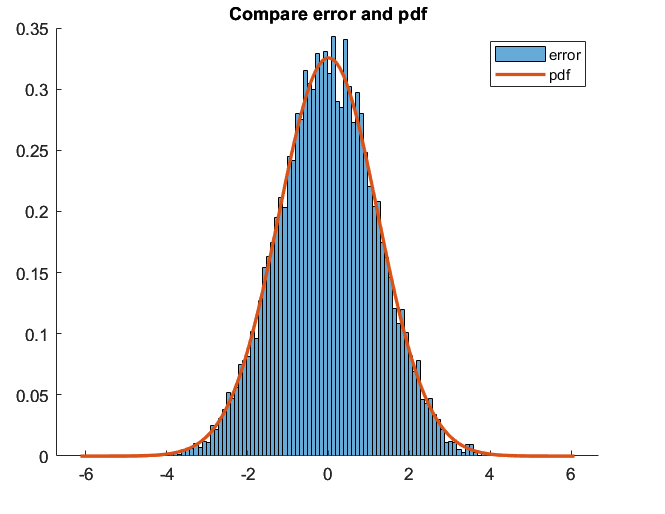
\includegraphics[width=0.7\textwidth]{images/higstogramandpdffor1e.png}
 \caption{Compare the histogram to the pdf $N(x;0, P_{N|N})$}
 \label{1e1}
\end{figure}

From figure \ref{1e1}, we can see after the normalization, the histogram matches the pdf curve.

This result supports the theory behind the Kalman filter that the estimation errors are normally distributed and that the filter provides optimal estimates with respect to the mean squared error criterion. Moreover, the fact that the histogram matches the expected pdf also suggests that the filter is working correctly and that the covariance matrix $P_{N|N}$ represents the uncertainty in the estimates well.

\subsubsection{Mean and Correlation of $v_k$}

From the lecture, the Kalman filter should have innovation consistency, which means $ v_k $ should satisfy:

\begin{equation}
    \begin{aligned}
        p(\textbf{v}_k\big|\textbf{y}_{1:k-1})&=\mathcal{N}(\textbf{v}_k;\textbf{0},\textbf{S}_k)\\
        Cov(v_k,v_{k-i})&=\begin{cases} cov\{v_k\}  & \text{if i=0}\\0 & \text{otherwise}\end{cases}\nonumber
    \end{aligned}
\end{equation}

Based on these two properties, I drew two pictures as in figure \ref{e21e22}.
\begin{figure}[H]
    \centering
    \begin{subfigure}[b]{0.45\textwidth}
        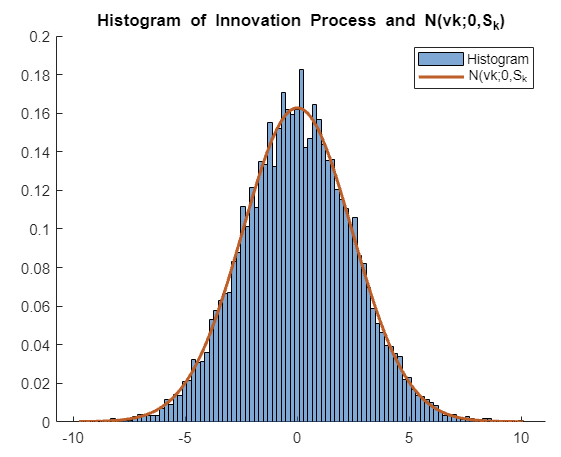
\includegraphics[width=\textwidth]{images/1e21.png}
        \caption{Histogram of Innovation Process and $N(v_k;0,S_k)$}
        \label{e21}
    \end{subfigure}
    \hfill
    \begin{subfigure}[b]{0.45\textwidth}
        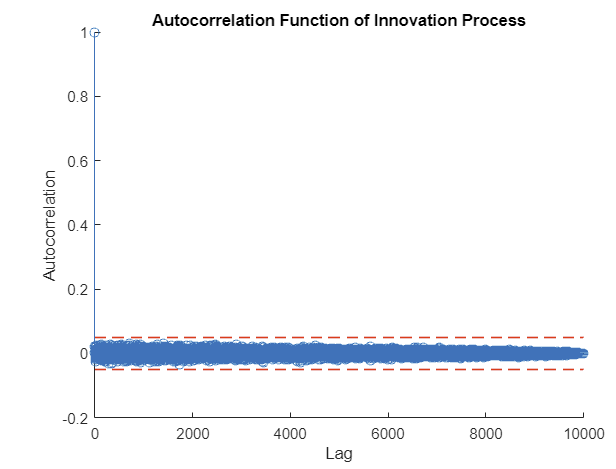
\includegraphics[width=\textwidth]{images/1e22.png}
        \caption{Autocorrelation Function of Innovation Process}
        \label{e22}
    \end{subfigure}
    \caption{Innovation Consistancy}
    \label{e21e22}
    \end{figure}
    
From figure \ref{e21}, we can see that the histogram of innovation process fits the pdf $N(v_k;0,S_k)$.

The two red lines in figure \ref{e22} are +/- 0.05, which shows that the innovations are not correlated except at the \emph{0} position, so it tells the process fits the property of cov.

Since the consistency condition is satisfied, it implies that the Kalman filter is optimal in the sense that it provides the best linear unbiased estimate of the state given the measurements and that the estimation error is the minimum mean square error.
